% document formatting
\documentclass[10pt]{article}
\usepackage[utf8]{inputenc}
\usepackage[left=1in,right=1in,top=1in,bottom=1in]{geometry}
\usepackage[T1]{fontenc}
\usepackage{xcolor}

% math symbols, etc.
\usepackage{amsmath, amsfonts, amssymb, amsthm}

% lists
\usepackage{enumerate}
\usepackage{multirow}

% images
\usepackage{graphicx} % for images

% code blocks
\usepackage{minted, listings} 

% verbatim greek
\usepackage{alphabeta}

\graphicspath{{./assets/images}}

\newcommand{\solution}{\textbf{Solution:}} 

\title{COM SCI M151B Week 2}

\author{Aidan Jan}
\date{\today}

\begin{document}
\section*{Microarchitecture}
\begin{itemize}
    \item The hardware implementation of ISA is called \textit{microarchitecture}
    \item A given ISA (e.g., RISC-V) can be implemented in many different ways (i.e., same ISA, different microarchitecture)
    \item The goal is to build an \textit{efficient} computer
    \begin{itemize}
        \item Fast (high performance) and power efficient.
    \end{itemize}
\end{itemize}

\subsection*{State-Machine View}
\begin{itemize}
    \item How do we make a microarchitecture?  
    \item There are two different parts:
    \begin{enumerate}
        \item Controller: a unit that directs the operation/activities on the datapath
        \item Data Path: a collection of \textit{functional} units that process the data and create the data-flow
    \end{enumerate}
\end{itemize}
\begin{center}
    \includegraphics*[scale=0.8]{W2_1.png}
    \includegraphics*[scale=0.8]{W2_2.png}
\end{center}
We will go through how this works, step by step.  But first, how are instructions executed?
\subsection*{Lifecycle of an instruction}
\begin{enumerate}
    \item Instruction is read (fetch) from the (instruction) memory
    \item Operands should be loaded
    \begin{itemize}
        \item RegFile, (data) Memory, Immediates
        \item Need register number / address for each operand
    \end{itemize}
    \item Operation should be executed
    \begin{itemize}
        \item Arithmetic (which type?), data movement, control-flow.
    \end{itemize}
    \item Results should be stored
    \begin{itemize}
        \item RegFile or memory?
    \end{itemize}
    \item PC should be updated
    \begin{itemize}
        \item Usually it is PC += 4, but sometimes it is different due to jumping/branching.
    \end{itemize}
\end{enumerate}
\subsubsection*{Instruction Fetch}
Provide a read address to the instruction, and get a 32 bit instruction.
\begin{center}
\includegraphics*[scale=0.8]{W2_3.png}
\end{center}
Registers stores data in a circuit. 
\begin{itemize}
    \item Uses a clock signal to determine when to update the stored value (could be multiple bits).
    \item Data stored in a register is read/written on the positive edge of the clock cycle.
    \item Uses D-flip-flop
    \item Some registers have a write-enable input.  If this is present, memory is only written when control input is 1.
\end{itemize}
Memory is an \textit{array of registers}.
\begin{itemize}
    \item Specific line can be chosen via a multiplexer.
\end{itemize}
\subsubsection*{Memory Technology}
\begin{itemize}
    \item Are all memory cells registers, SRAM, DRAM, etc.?
    \item No!
    \item \textbf{Latches and Flip-Flops (aka Registers)}
    \begin{itemize}
        \item Very fast (1 cycle), parallel access.
        \item Very expensive (one bit costs tens of transistors).
    \end{itemize}
    \item \textbf{Static RAM (SRAM)}
    \begin{itemize}
        \item Relatively fast (10 cycles), only one data word at a time.
        \item Expensive (one bit costs 6+ transistors).
    \end{itemize}
    \item \textbf{Dynamic RAM (DRAM)}
    \begin{itemize}
        \item Slower (100 cycles), one data word at a time, reading \textit{destroys} content (refresh), needs special process for manufacturing
        \item Cheap (one bit costs only one transistor plus one capacitor).
    \end{itemize}
    \item \textbf{DISK}
    \begin{itemize}
        \item flash memory, hard disk
        \item Much slower (1000+ cycles), access takes a long time
        \item Non-volatile
        \item Very cheap
    \end{itemize}
\end{itemize}
Which type of storage should we use?
\begin{itemize}
    \item From Register to DRAM to disk:
    \begin{itemize}
        \item From \textit{smaller} and \textit{faster} $\rightarrow$ \textit{bigger} and \textit{slower}
        \item From \textit{more expensive} and \textit{power hungry} $\rightarrow$ \textit{cheaper} and \textit{power efficient}
        \item The type we need depends on the purpose we need it for.  Use registers for frequently used data and slower and bigger elements for rarely-used permanent data.
    \end{itemize}
\end{itemize}
\subsubsection*{Loading Operands}
\begin{itemize}
    \item To load values from registers, we provide an address to read, with the write data bit at 0.  
    \item To write, we provide an address, the data to write, and the write enable bit.
    \item However, \textit{how could we know which instruction we read?}
    \begin{itemize}
        \item We need a controller!
    \end{itemize}
\end{itemize}
\begin{center}
    \includegraphics*[scale=0.5]{W2_4.png}
\end{center}
The controller directs the operations for each instruction.
\begin{center}
    \includegraphics*[scale=0.6]{W2_5.png}
\end{center}
We build controllers using finite state machines (FSMs).

\subsubsection*{Finite-State Machine (FSM)}
\begin{itemize}
    \item A \textit{mathematical} model of computation
    \item At each point, the system can be \textit{only at one} of the several, but \textbf{finite} states.
    \item FSM shows all the states and how they transit to each other.
    \item FSM also includes finite number of inputs and outputs.
\end{itemize}
\begin{center}
    \includegraphics*[scale=0.5]{W2_6.png}
    Remember these from CS181?
\end{center}
The FSM/Controller for a processor is simply a giant FSM with many states!
\begin{itemize}
    \item Lifecycle of each instructon in the controller:
    \begin{itemize}
        \item \textit{Initial State:} reading the instruction and decoding it.
        \item \textit{Next State:} each instruction has its own state.
        \item \textit{Future State:} depending on the instruction, there could be several states (e.g., reading registers, loading memory, arithmetic operations, etc.)
    \end{itemize}
    \item Once all the activities are done, the controller should go back to the \textit{initial state} and \textit{repeat} this process for the next instruction.
    \begin{itemize}
        \item We call this single-cycle design!
    \end{itemize}
\end{itemize}
\subsection*{Building a Simple CPU}
\begin{itemize}
    \item RISC-V ISA, 32-bit
    \item Handful of instructions - only 10
    \begin{itemize}        
        \item add, sub, and, or, lw, sw, beq, addi, andi, ori
    \end{itemize}
\end{itemize}
\subsubsection*{Creating nextPC}
Implement the part where you increment the program counter by 4.
\begin{center}
    \includegraphics*[scale=0.4]{W2_7.png}
\end{center}
\begin{itemize}
    \item Note that this will be modified later since we have branching, and not every instruction will increment by 4!
\end{itemize}
\subsubsection*{ALU}
\begin{center}
    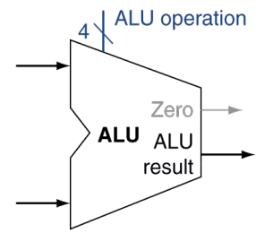
\includegraphics[scale=0.8]{W2_8.png}
\end{center}
ALU has two 32-bit inputs, an ALU result and Zero (x0) output, as well as a ALU operation with 4 bits, which selects the ALU operation to execute.
\subsubsection*{Register to ALU}
We need to connect the registers to the ALU.
\begin{center}
    \includegraphics*[scale=0.6]{W2_9.png}
\end{center}
\begin{itemize}
    \item The Immediate Generator takes in the bits of the instruction and shuffles it with the immediates to get the correct instruction format.  (funct7, rs2, rs1, funct3, rd, opcode, etc.)  Also does zero-padding if necessary.
    \item The registers provides the values in the registers that are needed.
    \item For R-type instructions without the need of immediates, the immediate generator generates garbage.  However, it does not matter since the MUX will not select it for the ALU.
\end{itemize}
\subsubsection*{Putting it all together}
\begin{center}
    \includegraphics*[scale=0.7]{W2_10.png}
\end{center}
The MemtoReg multiplexer decides whether data should be written.
\begin{itemize}
    \item This is the completed datapath used to execute an instruction.
    \item Now we need to wire it to the controller to pick which instruction to go to.
\end{itemize}
\begin{center}
    \includegraphics*[scale=0.6]{W2_11.png}
\end{center}
\begin{itemize}
    \item Notice that we added an additional MUX to pick whether to go to the next instruction (PC += 4), or branch somewhere else.
    \item The immediate generator also generates the offset in which to jump.
    \item We now have the datapath and the instruction selector, but still need a module to fill in the rest (control signals - blue wires).
\end{itemize}
\subsection*{Control Signals}
There are seven control signals:
\begin{itemize}
    \item RegWrite, ALUSrc, ALUOp, MemRead, MemWrite, MemtoReg, PCSrc
    \item This is where the finite state machine is used.
\end{itemize}
\subsubsection*{Control Signal FSM}
\begin{itemize}
    \item First, initialize the FSM state to zero.
    \item Based on the instruction (opcode), and current state, some control signals should be changed.
    \begin{itemize}
        \item First, we need to find out which instruction.  (Think: big opcode switch statement.  Include funct3 and funct7 if necessary)
        \item Once we know the instruction, we issue proper control signals (based on the list).
    \end{itemize}
\end{itemize}
\begin{center}
    \includegraphics*[scale=0.7]{W2_12.png}
\end{center}
\subsubsection*{Single-Cycle Design}
\begin{tabular}{|c|c|c|c|c|c|c|c|c|}
    \hline
    \textbf{Instruction} & \textbf{Opcode} & \textbf{RegWrite} & \textbf{AluSrc} & \textbf{Branch} & \textbf{MemRe} & \textbf{MemWr} & \textbf{MemtoReg} & \textbf{ALUOp}\\
    \hline
    R-type & 0110011 & 1 & 0 & 0 & 0 & 0 & 0 & -\\
    \hline
    I-type & 0010011 & 1 & 1 & 0 & 0 & 0 & 0 & -\\
    \hline
    lw & 0000011 & 1 & 1 & 0 & 1 & 0 & 1 & -\\
    \hline
    sw & 0100011 & 0 & 1 & 0 & 0 & 1 & 0 & -\\
    \hline
    beq & 1100011 & 0 & 0 & 1 & 0 & 0 & 0 & -\\
    \hline
\end{tabular}

\pagebreak
\noindent\textbf{ALUOp for each instruction:}\\
\begin{tabular}{|c|c|c|}
    \hline
    \textbf{Instruction} & \textbf{ALU Function} & \textbf{ALU Op}\\
    \hline
    lw & add & 0010\\
    \hline
    sw & add & 0010\\
    \hline
    beq & subtract & 0110\\
    \hline
    \multirow{4}{*}{R-type / I-type} & add & 0010 \\\cline{2-3}
                                     & subtract & 0110 \\\cline{2-3}
                                     & AND & 0000 \\\cline{2-3}
                                     & OR & 0001\\
    \hline
\end{tabular}
\subsection*{Dataflow with ALU Controller}
\begin{center}
    \includegraphics*[scale=0.75]{W2_13.png}
\end{center}

\section*{Efficiency}
\begin{itemize}
    \item The single-cycle processor is very simple and easy to design, but not the most efficient!  
    \item This is because different instructions have different paths and hence different delays.
    \item \textbf{Longest delay} determines clock period.
    \item The critical path is the \textit{load instruction}, which takes the longest: Instruction memory $\rightarrow$ register file $\rightarrow$ ALU $\rightarrow$ data memory $\rightarrow$ register file
    \item The only advantage of single-cycle designs is that they are simpler.
\end{itemize}
Can we do better?  How do we assess this?\\
\subsection*{Basic Metrics}
\begin{itemize}
    \item Latency
    \begin{itemize}
        \item How long does it take to finish a task (measured in sec, ms, $\mu$s, \dots)
        \item Lower is better
    \end{itemize}
    \item Throughput
    \begin{itemize}
        \item How many tasks can be done for a given time (measured in instruction per cycle, bit/second, \dots)
        \item Higher is better
    \end{itemize}
    \item Power
    \begin{itemize}
        \item Measured in J/sec
        \item Lower is better
    \end{itemize}
    \item Energy
    \begin{itemize}
        \item Product of power and latency (a function of both)
    \end{itemize}
\end{itemize}
\subsubsection*{Throughput vs. Latency}
Is $\text{throughput} = \frac{1}{\text{latency}}$?
\begin{itemize}
    \item If it takes $t$ seconds to do 1 task, then latency = $t$, does throughput = $1 / t$?
    \item If it takes $T$ seconds to do $N$ tasks, then throughput = $N / T$, does latency = $T / N$?
    \item If there is concurrency (e.g., running in parallel, then throughput $\neq$ 1 / latency).
\end{itemize}
\textbf{(Confusing) Terminology:}
\begin{itemize}
    \item Improved by 2.5x = improved by 150\% = improved by 2.5 times
    \item For \textit{bigger-is-better} metrics, "improved" means \textbf{increase}, but for \textit{smaller-is-better} metrics, "improved" means \textbf{decrease}
\end{itemize}

\subsection*{What is performance?}
\begin{itemize}
    \item \textbf{Time} is the measure of computer performance:
    \begin{itemize}
        \item The computer that performs the \textbf{same amount of work} in the \textbf{least time} is the fastest.
    \end{itemize}
\end{itemize}

\subsection*{Measuring Time in a Computer}
\begin{center}
    \includegraphics*[scale=0.6]{W2_14.png}
\end{center}
\begin{itemize}
    \item How to measure CPU Time?
    \begin{itemize}
        \item Directly: just run the program and measure time!  --\textit{too costly}
        \item Simulation: create a piece of software that accurately simulates the behavior of a real processor.  --\textit{architects love this!  But, there is a trade-off between simulation accuracy and complexity!}
    \end{itemize}
    \item What types of applications should be used?
    \begin{itemize}
        \item Different applications have different characteristics.
        \item Solution: Benchmarking
    \end{itemize}
\end{itemize}

\subsubsection*{Benchmark Software}
\begin{itemize}
    \item A set of programs that were carefully designed to measure a specific metric (usually CPU's performance).
    \item The purpose of benchmarking (depends on who you talk to)
    \begin{itemize}
        \item \textbf{The Architect:} Prove my gizmo is great!
        \item \textbf{Marketing:} Make us look good to sell \$\$ and crush our competition.
        \item \textbf{The Users:} Be our proxy, run our applications on new systems so we don't waste our money or our time.
    \end{itemize}
\end{itemize}

\subsubsection*{"Iron Law" of Processor Performance}
\[\text{CPU Time} = \text{InstructionCount} \times \text{CyclePerInstruction} \times \text{CycleTime}\]
\begin{itemize}
    \item InstructionCount
    \begin{itemize}
        \item IC
        \item Total number of instructions that we are executing (i.e., how large is the program)
        \item To optimize performance (i.e., reducing CPU Time) IC should be decreased by changing the algorithm or using a better compiler/ISA.
    \end{itemize}
    \item CyclePerInstruction
    \begin{itemize}
        \item CPI (also widely used is I/CPI=IPC, or MIPS = million instructions per second)
        \item Cycles needed to execute a given instruction
        \item CPI differs for different instructions (e.g., MULT vs. ADD) to optimize performance
        \item CPI should be decreased by using different \textit{architectural} techniques
    \end{itemize}
    \item CycleTime
    \begin{itemize}
        \item CT=I/F\_clk
        \item Faster clock rate decreases CT.
        \item Device and architecture-level techniques can be used to improve CT.
        \item Dennard and Moore's Laws
    \end{itemize}
\end{itemize}
\subsection*{MultiCycle/MultiStage}
\begin{itemize}
    \item Break down the datapath into multiple stages
    \item Each stage can be executed in one cycle.
    \item Using these stages we can break down the critical path, and hence increase the clock frequency.
    \item Intermediate values are stored in registers.
\end{itemize}
\subsubsection*{How does \textit{multicycle} improve performance?}
\begin{itemize}
    \item This reduces CycleTime, but also increases CPI.  What about overall performance?
\end{itemize}





\end{document}